%=====================================================================
%  用于图分类的矩阵残差图神经网络
%  中文对照稿 —— 与 IEEE 会议英文投稿稿结构、数据、图表一致
%  目标篇幅：6 页以内（含参考文献）
%  编译方式：xelatex -> bibtex -> xelatex -> xelatex
%=====================================================================
% 9pt keeps the Chinese companion within the same 6-page budget as the
% English submission; Chinese glyphs occupy more vertical space than Latin
% text at the same nominal size.
\documentclass[9pt,twocolumn]{extarticle}
\usepackage[UTF8]{ctex}

\usepackage[a4paper,top=1.8cm,bottom=1.9cm,left=1.7cm,right=1.7cm,columnsep=0.6cm]{geometry}
\usepackage{amsmath}
\usepackage{amssymb}
\usepackage{booktabs}
\usepackage{array}
\usepackage{graphicx}
\usepackage{url}
\usepackage[numbers,sort&compress]{natbib}
\usepackage[hidelinks]{hyperref}

% 与英文稿一致的浮动体间距
\setlength{\textfloatsep}{6pt plus 2pt minus 2pt}
\setlength{\floatsep}{6pt plus 2pt minus 2pt}
\setlength{\intextsep}{6pt plus 2pt minus 2pt}
\setlength{\abovecaptionskip}{3pt}
\setlength{\belowcaptionskip}{2pt}
\renewcommand{\arraystretch}{0.92}

\graphicspath{{../../}{../../figures/}{figures/}}

\renewcommand{\thefigure}{\arabic{figure}}
\renewcommand{\thetable}{\arabic{table}}
\renewcommand{\theequation}{\arabic{equation}}

\title{\textbf{用于图分类的矩阵残差图神经网络}\\[4pt]
{\large\mdseries 中文对照稿}}
\author{胡雪林 \quad 付晓琴\textsuperscript{*}\\[3pt]
{\small 柳州铁道职业技术学院，广西柳州 545000，中国}\\[2pt]
{\small \textsuperscript{*}通讯作者：fuxiaoqin@ltzy.edu.cn}}
\date{}

\begin{document}

\twocolumn[
\begin{@twocolumnfalse}
\maketitle
\begin{abstract}
\noindent 残差连接被广泛用于稳定图神经网络训练，但残差设计通常被简化为沿深度方向的一维选择。多分支图分类器打开了更丰富的设计空间：残差信息可以沿深度方向流动，可以在分支之间横向传递，也可以在分支--层的二维局部邻域中复用。本文将矩阵残差图神经网络（Matrix-Residual Graph Neural Networks）作为图分类中残差拓扑的受控研究框架。该模型族把隐藏状态表示在分支--层网格上，并比较五种信息流设计：普通消息传递、纵向残差复用、横向分支交换、局部矩阵残差复用，以及稀疏/门控矩阵复用。主实验在统一的训练协议下覆盖六个数据集、四种消息传递算子与五折图级评估，并辅以分支数消融、机制分析，以及覆盖五类图族、二至八分类的受控合成基准。实验表明，没有任何一种残差拓扑在所有数据集和算子上普遍最优；分支数消融呈现的是数据集相关的有效工作区间，而非单调的容量收益；合成基准显示简单基线在低类别任务上仍具竞争力，而随着结构类别粒度提高，矩阵残差复用的优势趋于稳定。因此，残差拓扑、分支数与残差过滤应当联合选择；矩阵式复用更适合被理解为一个可调的残差族，而不是对简单纵向或横向残差路径的通用替代。
\end{abstract}

\noindent\textbf{关键词：} 图分类；图神经网络；残差连接；多分支架构；矩阵残差复用
\vspace{1.0em}
\end{@twocolumnfalse}
]

\section{引言}
\label{sec:intro-zh}

图神经网络（Graph Neural Networks, GNN）通过反复聚合局部邻域信息来学习图表征~\cite{kipf2017gcn}。这种消息传递视角已成为图分类的标准工具，因为它能够在同一个可微模型中同时利用节点属性、局部连接结构和图层级结构~\cite{gilmer2017neural,wu2020comprehensive}。该建模范式并不局限于标准基准：图分类器已被用于依据接触图识别植物液泡蛋白~\cite{suiIdentificationPlantVacuole2023}，以及在植物知识图谱上传播功能注释~\cite{baongoImprovingPlantFunctional2025}。在这类任务中，图标签可能同时依赖局部模体和全局组织结构，因此有用的中间证据必须保留到图层级池化阶段~\cite{ying2018hierarchical}。

增加深度或加入并行分支可以扩展容量，但同时也会改变网络中的信息传输。深层 GNN 可能出现过平滑（over-smoothing），即节点表示随传播步数增加而趋于相似~\cite{li2018deeper,oono2020simple}；也可能出现过挤压（over-squashing），即远距离信息被压缩进尺寸受限的消息中~\cite{alon2020bottleneck,topping2021understanding}。这些问题对图层级预测尤为关键，因为最终读出依赖于到达池化阶段的中间表示质量。残差连接是应对上述困难的常见手段~\cite{he2016deep,bresson2017residual}，DropEdge 与 Jumping Knowledge 聚合也以在传播过程中保留有用信息为目标~\cite{rong2019dropedge,xu2018representation}。然而，残差连接通常仍被当作默认的逐层组件，而不是被研究的对象：大多数残差图分类器只在同一条流中沿深度方向复用信息。

一旦模型包含多个分支，沿深度的残差复用就只是其中一条可能路径。残差信息也可以在同一深度的相邻分支之间流动，或经由分支--深度的对角邻域传递。已有工作提升了消息传递算子、池化与高阶邻域混合的能力~\cite{abu2019mixhop,li2024graph}，但这些设计并未分离出残差路由这一问题本身：如果在某一深度上存在多个分支状态，模型应当只复用同一分支的前一状态、横向交换状态，还是在局部二维邻域中同时组合两个方向？

本文将残差复用作为分支--层网格上的结构化设计问题加以研究。核心问题不是是否应当存在跳跃连接，而是残差信号应当流向何处。该网格揭示了三种受控邻域：沿深度方向的纵向复用、相邻分支之间的横向交换，以及同时组合同分支、相邻分支和对角路径的矩阵式复用。稀疏/门控变体进一步检验矩阵残差流量是否应在注入前过滤。研究是刻意受控的：分类器、读出、折划分协议与骨干选项均保持不变，只有残差拓扑及其控制机制发生变化。近期的图模型可能通过同时改变多个组件获得更强的绝对性能~\cite{du2024densegnn}；本文则有意固定这些组件，使残差拓扑本身保持可识别性，这遵循了图分类公平比较协议同样的准则~\cite{errica2020fair,morris2020tudataset}。由于真实基准在结构类别粒度上的覆盖范围有限，我们补充了类别标签由结构参数生成的受控合成图族作为压力测试。

本文围绕三个研究问题展开。\textbf{RQ1：} 在共享的图分类协议下，残差拓扑是否影响性能？\textbf{RQ2：} 分支数、残差流量与机制如何解释性能变化？\textbf{RQ3：} 在真实数据与受控合成多分类结构上，矩阵式残差复用何时更有效？主要贡献如下。

\begin{itemize}
\item \textbf{分支--层形式化。} 把纵向、横向、矩阵以及稀疏/门控矩阵残差族统一表达为同一网格上的局部邻域，使其信息流差异显式化。
\item \textbf{受控的真实数据与合成基准。} 所有比较的分类器、读出、折划分协议与骨干选择保持一致，并补充覆盖五类受控图族、二至八分类的结构压力测试。
\item \textbf{带有保守复验的机制分析。} 在报告精度的同时分析分支多样性、分支余弦相似度、中心核对齐（CKA）、梯度范数与残差活跃度；灵敏度扫描仅用于候选发现，选定配置需跨折复验后才作为实证结论。
\end{itemize}

\section{相关工作}
\label{sec:related-zh}

\textbf{消息传递。} 现代图学习建立在 Kipf 和 Welling 的谱卷积之上~\cite{kipf2017gcn}。GraphSAGE 引入归纳式邻域聚合~\cite{hamilton2017inductive}，图注意力网络以学习到的注意力对邻居加权~\cite{velivckovic2017graph}，消息传递神经网络框架则把上述设计统一用于分子性质预测~\cite{gilmer2017neural}。GIN 建立的 Weisfeiler--Lehman 联系说明单射多重集聚合是该族判别能力的关键~\cite{xu2019gin}，综述文献梳理了由此形成的设计空间~\cite{wu2020comprehensive}。

\textbf{深层 GNN 与残差连接。} 在消息传递中加深网络并非没有代价：过平滑使节点表示随传播深度增加而收敛~\cite{li2018deeper,oono2020simple}，过挤压则把远距离信息压缩进固定尺寸的消息~\cite{alon2020bottleneck,topping2021understanding}。DropEdge 在训练时随机移除边~\cite{rong2019dropedge}，Jumping Knowledge 聚合跨层表示~\cite{xu2018representation}，残差或稠密跳跃路径把早期状态向前传递~\cite{he2016deep}。残差门控图卷积网络学习历史状态应以多强的权重重新注入~\cite{bresson2017residual}。这些方法都在单条流内复用沿深度的状态；本文保留同样的复用原则，但提出不同的问题：分支--层网格上的哪些局部残差邻域应当被连接。

\textbf{多分支与高阶架构。} 高阶邻域混合优于单跳聚合~\cite{abu2019mixhop}。层次池化通过在处理过程中粗化图引入了第二个结构维度~\cite{ying2018hierarchical}，近期综述对由此形成的设计进行了归纳~\cite{li2024graph}。这些工作提升的是传播层的表达能力或聚合能力。与之不同，本文固定传播算子，只改变隐藏状态的复用方式，从而使残差拓扑本身成为可识别的因素。

\section{方法}
\label{sec:method-zh}

\subsection{符号与共享流程}
\label{sec:pipeline-zh}

设 \(\mathcal{G}=(\mathcal{V},\mathcal{E})\) 为图，节点特征矩阵为 \(\mathbf{X}\in\mathbb{R}^{n\times d_{\mathrm{in}}}\)，邻接结构为 \(\mathbf{A}\)。对于数据集 \(\mathcal{D}=\{(\mathcal{G}_i,y_i)\}_{i=1}^{N}\)，目标是学习 \(f_{\theta}:\mathcal{G}\rightarrow \hat{y}\)，其中 \(\hat{y}\) 为预测的图标签。设 \(B\) 为分支数，\(L\) 为消息传递层数，分支 \(b\)、层 \(\ell\) 处的隐藏状态记为 \(\mathbf{H}^{(\ell)}_{b}\)，其中 \(b\in\{1,\ldots,B\}\)。分支局部传播步为
\begin{equation}
\mathbf{Z}^{(\ell)}_{b} =
\phi^{(\ell)}_{b}\left(\mathbf{H}^{(\ell-1)}_{b}, \mathbf{A}\right),
\label{eq:prop-zh}
\end{equation}
其中 \(\phi\) 实例化为四种标准算子之一：GCNConv~\cite{kipf2017gcn}、GATConv~\cite{velivckovic2017graph}、SAGEConv~\cite{hamilton2017inductive} 或 GINConv~\cite{xu2019gin}。残差增强更新为
\begin{equation}
\mathbf{H}^{(\ell)}_{b} =
\mathbf{Z}^{(\ell)}_{b} +
\sum_{(b',\ell')\in\mathcal{N}(b,\ell)}
\mathcal{R}_{(b',\ell')\rightarrow(b,\ell)}
\left(\mathbf{H}^{(\ell')}_{b'}\right).
\label{eq:update-zh}
\end{equation}
在不同架构之间唯一变化的项是残差邻域 \(\mathcal{N}(b,\ell)\) 与残差变换 \(\mathcal{R}\)。在最后一个消息传递层之后，每个分支经全局平均池化得到图层级向量，再在分类前融合各分支向量，以交叉熵损失训练。我们有意避免可微池化等架构专用读出结构~\cite{ying2018hierarchical}，因为目的是分离残差拓扑，而非比较读出机制。图~\ref{fig:architecture-zh} 汇总了共享流程与本文比较的残差路径。选取这四种算子，是因为它们分别代表谱式卷积、基于注意力的聚合、邻域采样与聚合，以及单射多重集聚合。

\begin{figure}[!t]
\centering
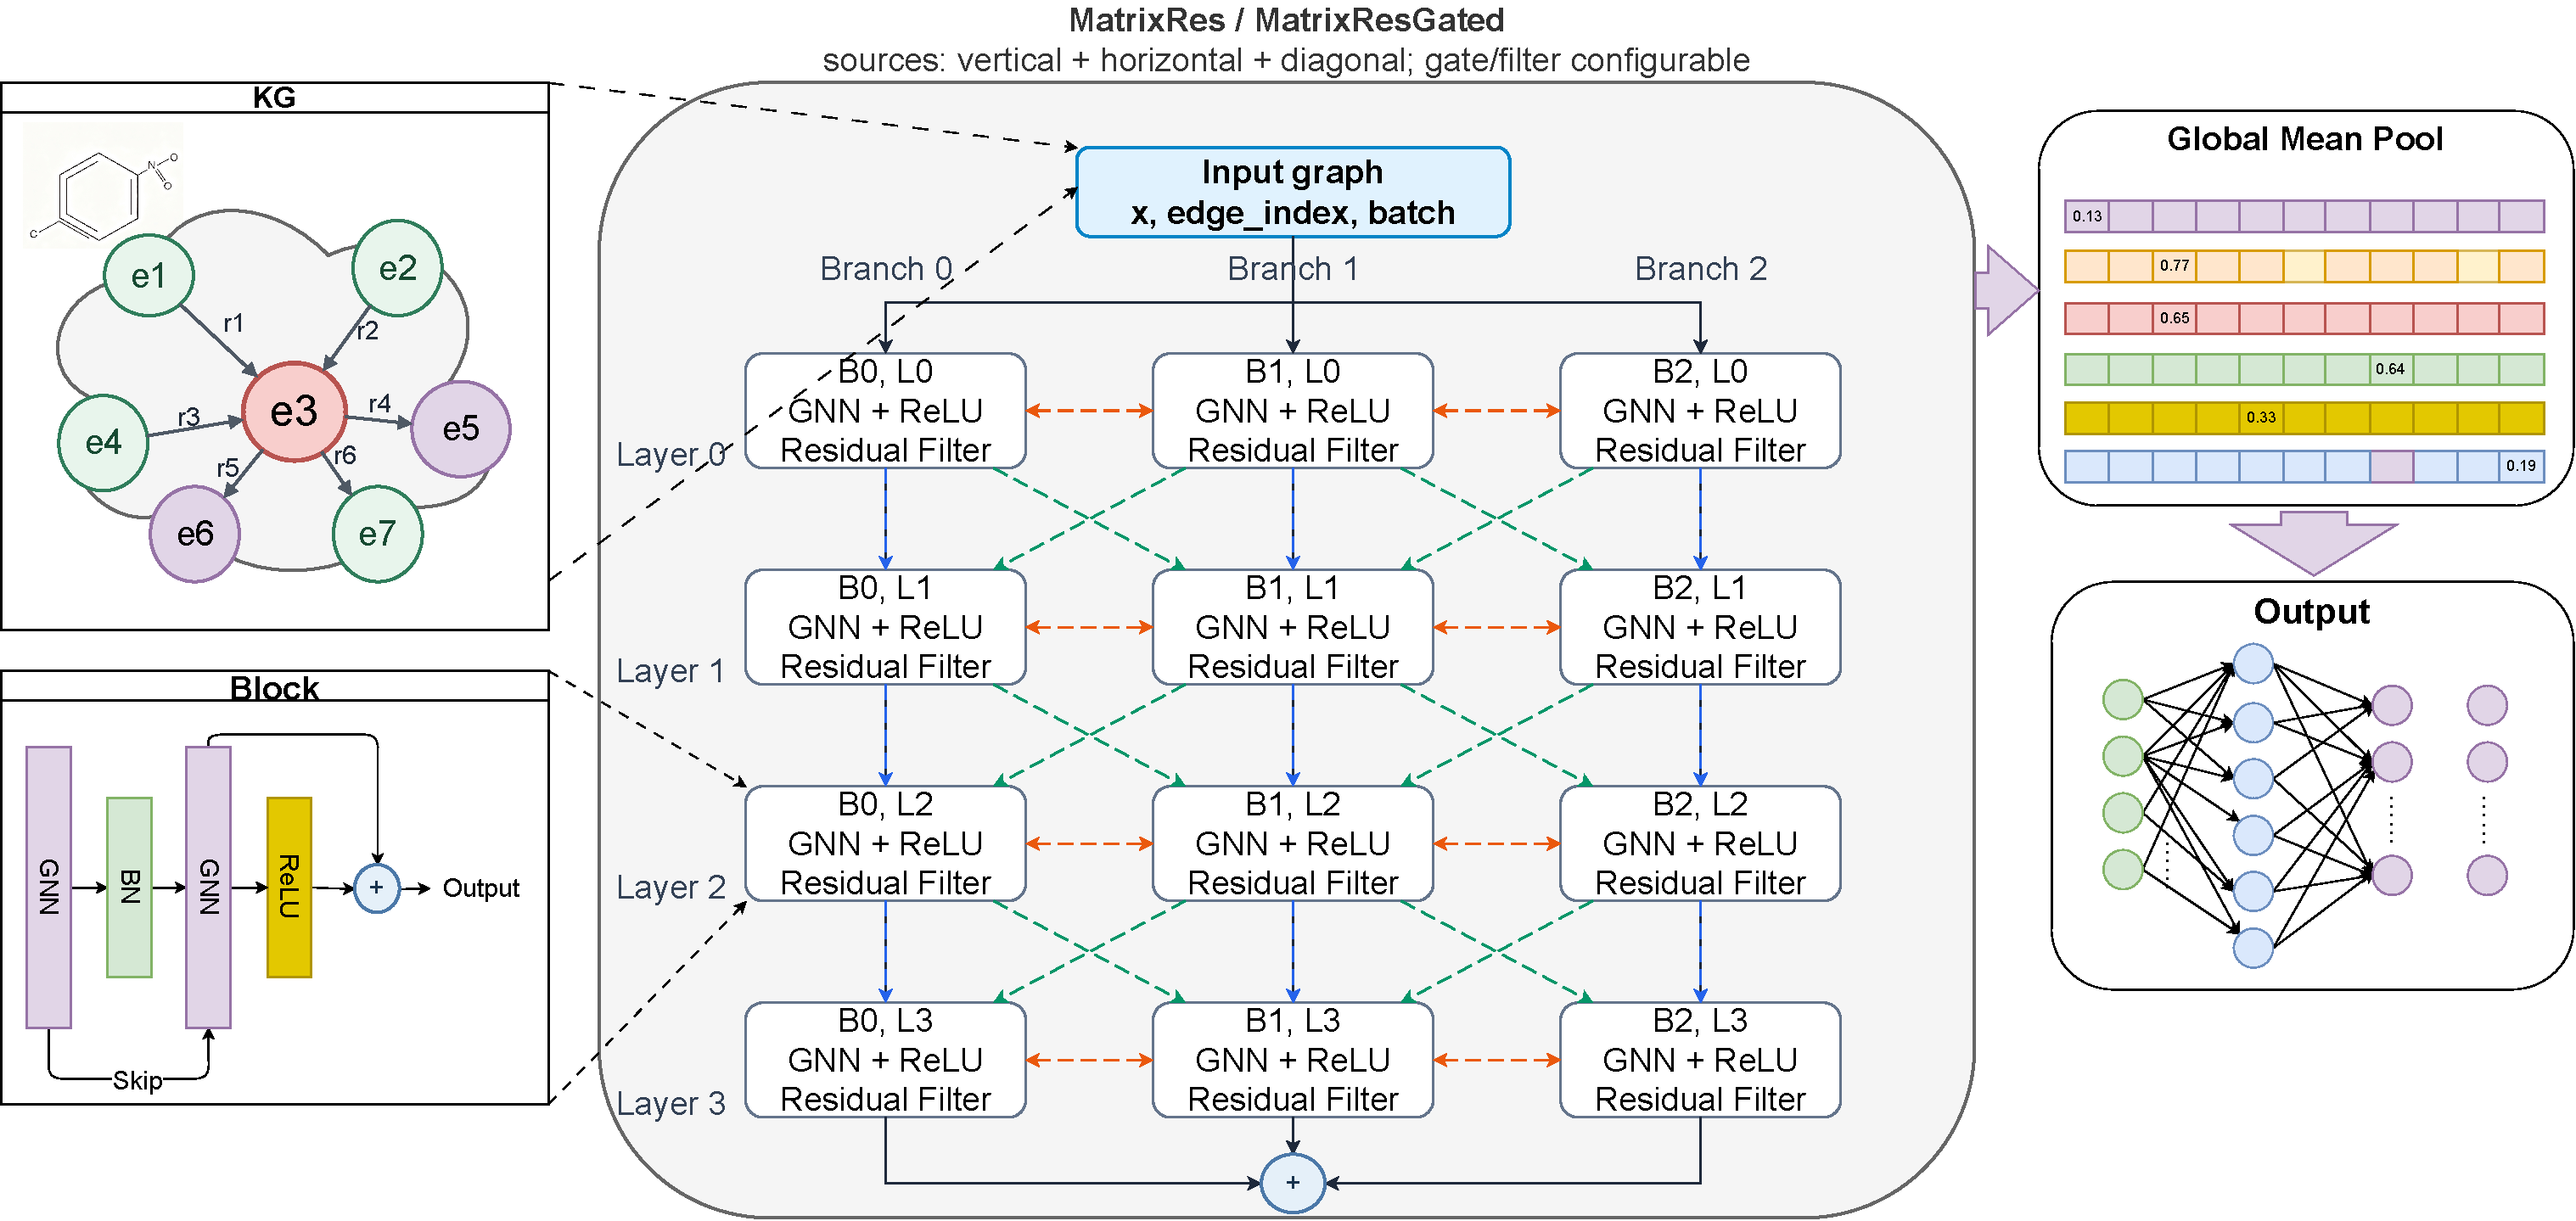
\includegraphics[width=0.98\linewidth]{figures/cr_gnn_graph_architecture.pdf}
\caption{分支--层网格上各残差邻域的架构概览。消息传递骨干与图层级读出保持不变，仅改变残差路径。}
\label{fig:architecture-zh}
\end{figure}

\subsection{残差邻域}
\label{sec:model-zh}

\textbf{Plain} 不含残差邻域，\(\mathcal{N}(b,\ell)=\emptyset\)。\textbf{VerticalRes} 注入同一分支的上一层，\(\mathcal{N}(b,\ell)=\{(b,\ell-1)\}\)。\textbf{HorizontalRes} 在同一深度上交换相邻分支的信息，\(\mathcal{N}(b,\ell)=\{(b-1,\ell),(b+1,\ell)\}\)，边界分支只使用有效邻居；当 \(B=1\) 时该邻域为空。\textbf{MatrixRes} 同时组合纵向、横向与对角邻域：
\begin{equation}
\mathcal{N}(b,\ell)=
\{(b,\ell-1),(b-1,\ell),(b+1,\ell),(b-1,\ell-1),(b+1,\ell-1)\}.
\label{eq:matrix-zh}
\end{equation}
该局部模板有意不采用稠密的全连接混合，而是在分支--层网格上保留可解释的残差结构。无效的边界邻居会被移除，因此当 \(B=1\) 时，MatrixRes 在首层之后仍保留同分支纵向残差路径，但不含分支邻居路径。

\textbf{MatrixResGated} 使用相同邻域，但通过残差变换控制注入信号：
\begin{equation}
\mathcal{R}(\mathbf{U}) =
\begin{cases}
\alpha \mathbf{U}, & \text{带门控的恒等过滤},\\[2pt]
\alpha\,\mathrm{softshrink}_{\lambda}(\mathbf{U}), & \text{带门控的稀疏过滤}.
\end{cases}
\label{eq:gate-zh}
\end{equation}
Plain、VerticalRes、HorizontalRes 与 MatrixRes 使用恒等残差过滤。MatrixResGated 使用稀疏过滤，\(\lambda=0.05\)，可学习标量门初始化为 0.8；当 \(B=1\) 时仍对其余矩阵残差路径施加门控稀疏过滤。实现同样支持 top-\(k\) 过滤与固定门，但主结果未使用。

\subsection{实验设置}
\label{sec:setup-zh}

主实验使用通过 PyTorch Geometric 访问的六个 TUDataset 数据集~\cite{morris2020tudataset,fey2019fast}：PROTEINS、DD、ENZYMES、MUTAG、AIDS 与 Mutagenicity。PROTEINS 与 DD 是二分类蛋白质结构任务，ENZYMES 为六分类，MUTAG、AIDS 与 Mutagenicity 提供分子图稳健性检验。图以其自带特征加载；不使用手工描述子、图增强或边重连，使比较反映残差拓扑而非特征工程。

全部结果采用图级五折评测。对第 \(k\) 折，测试精度为 \(\mathrm{Acc}_{k}=|\mathcal{T}_{k}|^{-1}\sum_{(\mathcal{G}_{i},y_{i})\in\mathcal{T}_{k}}\mathbf{1}[\hat{y}_{i}=y_{i}]\)，并报告跨折均值与折级标准差。精度作为主指标，是因为所有基准都有离散的图标签。合成基准额外报告对每类等权的宏平均 F1，以及随机归一化精度 \(\mathrm{NAcc}=(\mathrm{Acc}-1/C)/(1-1/C)\)，因为原始精度在类别数变化时不可直接比较。分支多样性、余弦相似度、CKA、残差活跃度与梯度范数等机制指标用作诊断，而非优化目标。

为在受控结构粒度下检验残差拓扑，我们构建了基于五类图族的合成基准：伯努利随机图（ER）、Barab\'asi--Albert（BA）图、随机块模型（SBM）~\cite{holland1983stochastic}、Watts--Strogatz（WS）图~\cite{watts1998collective}，以及规则度对照。对每一图族生成 \(C\in\{2,\ldots,8\}\) 的七个数据集，每类 200 张图，图规模 30--80 个节点。节点特征为归一化度数与随机通道导出的八维向量，不编码类别标签。标签由图族特定的结构参数控制：ER 由边概率控制~\cite{gilbert1959random}，BA 由优先连接数控制~\cite{barabasi1999emergence}，SBM 由块内与块间概率控制，WS 由重连概率控制，规则度对照由固定度数控制。这些图族用作压力测试，而非真实基准的替代。

表~\ref{tab:hyperparams-zh} 列出共享设置。分支数消融在 GCNConv 下对 PROTEINS 与 DD 评估 HorizontalRes、MatrixRes 与 MatrixResGated 的 \(B=1,\ldots,8\)。灵敏度扫描在 \(B=3\) 下对 fold 0 进行，变化学习率、dropout、隐藏维度、稀疏强度与门初始化；选定候选随后在全五折上复验。实验运行于配备 AMD Ryzen 7 5700X CPU 与 NVIDIA RTX 3090 GPU 的 Ubuntu 服务器。

\begin{table}[!t]
\centering
\caption{关键实验设置}
\label{tab:hyperparams-zh}
\footnotesize
\begin{tabular}{@{}p{0.36\linewidth}p{0.56\linewidth}@{}}
\toprule
参数 & 取值 \\
\midrule
消息传递算子 & GCNConv、GATConv、SAGEConv、GINConv \\
分支数 / 层数 & \(B=3\)；\(L=4\)（DD 为 \(L=3\)） \\
隐藏维度 & 64 \\
评测方式 & 五折图分类 \\
Plain/Vertical/Horizontal & 200 轮，patience 60，lr 0.005，权重衰减 \(10^{-4}\)，dropout 0.5 \\
MatrixRes/MatrixResGated & 240 轮，patience 80，lr 0.003，权重衰减 \(5\times10^{-5}\)，dropout 0.3 \\
学习率调度 & ReduceLROnPlateau，factor 0.5，patience 15，最小 lr \(10^{-5}\) \\
梯度裁剪 & 范数 2.0 \\
\bottomrule
\end{tabular}
\end{table}

\section{实验结果}
\label{sec:results-zh}

除特别说明外，全部结果以五折平均最优测试精度 \(\pm\) 折级标准差报告。

\subsection{整体基准表现}

主实验检验的是：在数据集与算子之间是否存在稳定的残差拓扑赢家。答案是否定的。在 24 个数据集--算子组合中（表~\ref{tab:operator_wins-zh}），MatrixRes 获胜最频繁，取得 9 次胜利并具有最佳平均排名（2.12）；MatrixResGated 与 Plain 各获胜 5 次，HorizontalRes 获胜 3 次，VerticalRes 获胜 2 次。因此矩阵式复用具有最有利的总体表现，但每种拓扑都在某些设置下最强。各数据集的获胜者较为混杂：矩阵族在 MUTAG、AIDS 与 Mutagenicity 上占优，而 PROTEINS 在 Plain 与 HorizontalRes 之间交替，DD 在 HorizontalRes、MatrixRes 与 VerticalRes 之间交替。ENZYMES 仍然困难，未出现稳定偏好。

\begin{table}[!t]
\centering
\caption{24 个数据集--算子组合上的获胜次数与平均排名}
\label{tab:operator_wins-zh}
\footnotesize
\begin{tabular}{@{}lccc@{}}
\toprule
模型 & 获胜次数 & 平均排名 & GCNConv 获胜 \\
\midrule
Plain          & 5 & 3.04 & PROTEINS \\
VerticalRes    & 2 & 3.38 & --- \\
HorizontalRes  & 3 & 3.54 & DD \\
MatrixRes      & \textbf{9} & \textbf{2.12} & MUTAG、AIDS、Mutagenicity \\
MatrixResGated & 5 & 2.92 & ENZYMES \\
\bottomrule
\end{tabular}
\end{table}

ENZYMES 需谨慎解读，因为所有模型的绝对精度都很低。剔除 ENZYMES 后，MatrixRes 在 20 个组合中仍取得 9 次胜利，平均排名为 2.05，总体偏好不变。

为排除算子带来的差异，我们单独报告 GCNConv 切片（表~\ref{tab:main_benchmark-zh}、图~\ref{fig:main_benchmark-zh}）。结论一致：MatrixRes 在 MUTAG、AIDS 与 Mutagenicity 上最强，而更简单的残差路径在 PROTEINS、DD 与 ENZYMES 上仍然更优。残差拓扑确实重要，但其价值取决于数据集。

\begin{table}[!t]
\centering
\caption{\(B=3\) 下的 GCNConv 基准（五折平均）}
\label{tab:main_benchmark-zh}
\footnotesize
\begin{tabular}{@{}lccccc@{}}
\toprule
数据集 & Plain & Vertical & Horizontal & Matrix & MatrixGated \\
\midrule
PROTEINS     & \(\mathbf{0.7044}\) & 0.6993 & 0.6992 & 0.6973 & 0.6886 \\
DD           & 0.7053 & 0.7143 & \(\mathbf{0.7181}\) & 0.7127 & 0.7141 \\
ENZYMES      & 0.2683 & 0.2550 & 0.2633 & 0.2750 & \(\mathbf{0.2933}\) \\
MUTAG        & 0.7556 & 0.7451 & 0.7343 & \(\mathbf{0.7609}\) & 0.7556 \\
AIDS         & 0.8215 & 0.8210 & 0.8130 & \(\mathbf{0.8365}\) & 0.8150 \\
Mutagenicity & 0.7644 & 0.7667 & 0.7738 & \(\mathbf{0.7784}\) & 0.7701 \\
\bottomrule
\end{tabular}
\end{table}

\begin{figure}[!t]
\centering
\includegraphics[width=0.98\linewidth]{figures/exp/fig_main_benchmark_gcnconv.pdf}
\caption{\(B=3\) 下的 GCNConv 基准。各单元格折级标准差介于 0.005 与 0.072 之间。}
\label{fig:main_benchmark-zh}
\end{figure}

\subsection{合成多分类缩放}

合成基准检验的是：在受控图生成规则下提高结构类别粒度时，残差拓扑的行为是否改变。表~\ref{tab:synthetic_class_scaling-zh} 汇总了对五个图族与四种算子取平均后的趋势。低类别设置并不偏好矩阵式复用：\(C=2\) 时 Plain 最优，\(C=3\) 时 HorizontalRes 最优。从 \(C=4\) 起矩阵式复用变得更有竞争力，MatrixResGated 在 \(C=4\)、\(C=5\)、\(C=6\) 与 \(C=8\) 上是最强的平均精度模型。在高类别区间 \(C=4,\ldots,8\)，MatrixResGated 达到 0.6943 精度与 0.6324 归一化精度，而 Plain 为 0.6827 与 0.6183；MatrixRes 具有最佳宏平均 F1（0.6880）。MatrixRes 从 \(C=2\) 到 \(C=8\) 的精度下降也最小（0.3479，Plain 为 0.3720），说明稠密局部矩阵复用随标签空间变细而相对稳定。

\begin{table}[!t]
\centering
\caption{对五个图族与四种算子取平均的合成缩放}
\label{tab:synthetic_class_scaling-zh}
\footnotesize
\begin{tabular}{@{}clcccc@{}}
\toprule
类别数 & 最优模型 & Plain & Matrix & MatrixGated & 最优 NAcc \\
\midrule
2 & Plain          & \(\mathbf{0.9585}\) & 0.9481 & 0.9578 & 0.9170 \\
3 & HorizontalRes  & 0.8774 & 0.8600 & 0.8772 & 0.8200 \\
4 & MatrixResGated & 0.8002 & 0.8083 & \(\mathbf{0.8111}\) & 0.7481 \\
5 & MatrixResGated & 0.7233 & 0.7280 & \(\mathbf{0.7296}\) & 0.6621 \\
6 & MatrixResGated & 0.6719 & 0.6827 & \(\mathbf{0.6878}\) & 0.6254 \\
7 & VerticalRes    & 0.6314 & 0.6429 & 0.6395 & 0.5945 \\
8 & MatrixResGated & 0.5865 & 0.6002 & \(\mathbf{0.6035}\) & 0.5469 \\
\bottomrule
\end{tabular}
\end{table}

\begin{figure}[!t]
\centering
\includegraphics[width=0.98\linewidth]{figures/exp/fig_synthetic_multiclass_scaling.pdf}
\caption{从二分类到八分类的合成缩放，对五个图族与四种算子取平均。}
\label{fig:synthetic_multiclass_scaling-zh}
\end{figure}

在图族层面，MatrixRes 在高类别数的 BA、ER 与规则度设置中最强，这些设置的标签分别与度数增长、边概率或度均匀结构变化相关。这些图族具有共同模式：标签空间由彼此相关的结构区间构成，而非互不相关的类别，因此局部矩阵复用可以把沿深度的细化与相邻分支交换结合起来。SBM 由社区驱动，对矩阵式复用相对不利，但 MatrixRes 仍接近最佳结果。

\subsection{分支数消融与机制分析}

分支数不只是容量参数，它同时改变残差路径密度。表~\ref{tab:branch_best-zh} 报告每种拓扑的最佳与最差分支数。在 PROTEINS 上有效区间较为适中（HorizontalRes 在 \(B=4\)、MatrixRes 在 \(B=6\)、MatrixResGated 在 \(B=3\) 达到峰值）；在 DD 上有效区间更小（HorizontalRes 与 MatrixRes 在 \(B=2\) 达到峰值，MatrixResGated 在 \(B=1\) 时已最强）。因此分支扩展并非单调，必须与任务结构相匹配。

\begin{table}[!t]
\centering
\caption{分支数消融：最佳与最差设置}
\label{tab:branch_best-zh}
\footnotesize
\begin{tabular}{@{}llcccc@{}}
\toprule
数据集 & 模型 & 最佳 \(B\) & 最佳精度 & 最差 \(B\) & 最差精度 \\
\midrule
PROTEINS & HorizontalRes  & 4 & \(\mathbf{0.7125}\) & 1 & 0.6801 \\
PROTEINS & MatrixRes      & 6 & \(\mathbf{0.7062}\) & 1 & 0.6909 \\
PROTEINS & MatrixResGated & 3 & \(\mathbf{0.7098}\) & 4 & 0.6711 \\
DD       & HorizontalRes  & 2 & \(\mathbf{0.7275}\) & 4 & 0.7071 \\
DD       & MatrixRes      & 2 & \(\mathbf{0.7206}\) & 7 & 0.7071 \\
DD       & MatrixResGated & 1 & \(\mathbf{0.7283}\) & 7 & 0.7053 \\
\bottomrule
\end{tabular}
\end{table}

\begin{figure}[!t]
\centering
\includegraphics[width=0.98\linewidth]{figures/exp/fig_branch_count_ablation.pdf}
\caption{GCNConv 下 PROTEINS 与 DD 的分支数消融。精度只在有效工作区间内提升，随后趋于饱和或下降。}
\label{fig:branch_ablation-zh}
\end{figure}

机制指标解释了这一分化。在 PROTEINS 上，HorizontalRes 从 \(B=1\) 提升到 \(B=4\)，分支多样性由 0.0000 升至 1.1450，分支余弦由 1.0000 降至 0.8417；但多样性本身并不充分：\(B=8\) 时多样性进一步升至 1.5441，精度却降至 0.6881。MatrixRes 在更大尺度上呈现同一规律，在 \(B=6\) 达到峰值，多样性为 3.7755。在 DD 上，最佳设置的分支余弦已接近饱和（\(B=2\) 时 HorizontalRes 为 0.9969，MatrixRes 为 0.9991），CKA 为 1.0000，因此额外的残差流量难以产生新的功能分离；更大的分支数提升了多样性却未改善精度。MatrixResGated 表现为真正的残差控制而非稠密路径：其活跃比例在 PROTEINS 最佳设置下为 0.3121，在 DD 最佳设置下为 0.2352，同时学习到的门保持在 0.78--0.84 附近而非塌缩为零。以上均为诊断性相关分析，而非因果干预。门控变体并未在总体上压过 MatrixRes，因此稀疏过滤最好被视为一种流量控制机制，而非普适改进。

\subsection{灵敏度与五折验证}

fold-0 扫描只用于候选发现。在 PROTEINS 上，MatrixRes 在测试的扫描范围内未超过其 fold-0 基线，而 MatrixResGated 存在一个轻稀疏候选（\(\lambda=0.02\) 把 fold-0 精度从 0.6726 提升至 0.6951；更强的稀疏化则有害）。在 DD 上两种模型都偏好更小的隐藏维度，分别在 \(d=32\) 时达到 0.7595 与 0.7511。把选定候选在全五折上复验可避免过度断言：在 DD 上，\(d=32\) 的 MatrixResGated 候选保持竞争性（\(0.7215\pm0.0330\)），同时把参数量从 42{,}371 降至 15{,}043；而在 PROTEINS 上，稀疏候选未能在各折上保持其 fold-0 优势（\(0.6909\pm0.0447\)），仍属不稳定候选，而非已确认的增益。

\section{讨论}
\label{sec:discussion-zh}

\subsection{RQ1：残差拓扑与性能}

主实验不支持存在通用残差拓扑：MatrixRes 获胜最频繁且平均排名最佳，但五种模型族都至少赢得 24 个组合中的两个，GCNConv 切片同样呈现数据集相关的获胜者。因此有用的残差邻域取决于数据集对分支特化、残差流量与优化复杂度的容忍度。这与更广泛的文献一致：改变传播算子、归一化或池化设计往往会改变首选架构~\cite{xu2019gin,hamilton2017inductive,ying2018hierarchical}。本文补充的发现是：残差拓扑本身也是这种变化的来源之一。矩阵式复用可以理解为分支--层网格上的局部残差模板，其精神类似结构化邻域混合~\cite{abu2019mixhop}，但作用于隐藏状态复用而非图邻接；它的优势来自架构组织方式，而不是新的消息传递原语。

\subsection{RQ2：分支数与机制}

增大 \(B\) 会同时增加分支、残差路径与优化交互，因此不是简单的容量旋钮。PROTEINS 能够承受适中的分支预算（峰值在 \(B=4\)--\(6\)），而 DD 偏好 \(B=1\)--\(2\)。机制指标与这一分化一致：在 PROTEINS 上，最佳设置同时具备更高的分支多样性与更低的余弦；在 DD 上，最佳设置的余弦与 CKA 已接近饱和，额外的残差流量难以产生新功能。多样性可能随 \(B\) 增大，但当分支相似度仍然很高或梯度减弱时，它本身并不能改善分类。这种先升后降的行为对残差 GNN 设计是一个实践警示，因为残差连接常被引入以使更深或更宽的模型更易优化~\cite{he2016deep}。功能多样性与残差干扰之间的平衡在两个通常都被视为蛋白质结构基准的数据集之间差异显著。

\subsection{RQ3：矩阵式复用何时有益}

稀疏/门控复用并不普遍优于稠密矩阵复用：MatrixRes 总体上赢得更多组合。MatrixResGated 仍然有用，因为它提供了一种受控地抑制弱残差系数的方式，机制分析也证实它比稠密 MatrixRes 保留更少的活跃通路，同时门保持在中等水平。其价值不在于稀疏总能提升精度，而在于当矩阵复用否则会注入过多低价值流量时，过滤是有益的。这把它置于两种已有思想之间：与残差门控图网络类似，它学习历史信息应以多强权重注入~\cite{bresson2017residual}；与稀疏化方法类似，它削弱弱路径的影响~\cite{rong2019dropedge}。实现刻意保持简单——使用标量门与软阈值过滤，而非大型路由网络——以保持消融的可解释性。候选设置仍须跨折验证：DD 的隐藏维度候选通过了检验并得到更小、更高效的模型，而 PROTEINS 的稀疏候选未能通过，不应被宣称是增益。

合成基准把类别粒度与真实数据集的特殊性分离开来。在二分类与三分类上，简单的残差选择仍具竞争力，这避免了"矩阵式复用总被需要"这一过宽论断。从四分类起模式逆转：MatrixResGated 具有最佳平均精度与归一化精度，MatrixRes 具有最佳宏平均 F1 以及从 \(C=2\) 到 \(C=8\) 的最小降幅。分布层面的结果进一步表明：MatrixRes 在度数驱动与密度驱动的 BA、ER 与规则度图族中领先，这些图族的标签区分的是彼此相关的结构区间而非互不相关的类别；而由社区驱动的 SBM 则相对不利。综合来看，矩阵式复用是条件性有效而非通用的，并且在任务需要在更细的判别下区分若干相关结构区间时最为有用。

\subsection{局限性}

以下几点限制了结论的普适性。基准使用固定的图层级池化与分类头，因此其他读出设计可能与残差拓扑产生交互。所比较的算子是经典消息传递骨干，而非近期的图 Transformer 或局部--全局混合架构~\cite{dwivedi2020generalization}，这是刻意的控制选择，但也意味着本文不是最先进模型的比较。灵敏度扫描仅在 fold 0 上进行，候选复验也仅覆盖 PROTEINS 与 DD 上的 MatrixResGated。ENZYMES 的绝对精度低且波动大。机制分析属于相关性分析：分支多样性、余弦相似度、CKA 与梯度范数支持一个自洽的解释，但并不证明因果性。最后，基准有意避免任务专用的化学或生物特征工程，因此绝对精度不应被解读为经过优化的最先进分子预测结果，合成图族也只是用于压力测试残差拓扑，而非替代更广泛的真实多分类基准。未来工作应把比较扩展到更大的数据集、更丰富的读出机制、近期的局部--全局骨干，以及可学习残差邻域策略，以替代人工指定的纵向、横向与矩阵模板。

\section{结论}
\label{sec:conclusion-zh}

本文将图分类中的残差连接研究为结构化的分支--层设计问题。在六个数据集与四种消息传递算子上，残差拓扑确实重要，但其价值取决于数据集、算子与分支预算。MatrixRes 在完整基准中获胜最频繁且平均排名最佳，但各数据集的 GCNConv 获胜者仍然混杂，且 ENZYMES 的绝对精度较低，应谨慎解读。分支数消融表明，增加分支只在一个有限的工作区间内有用：额外分支提高表示多样性，但同时也增加残差流量，并可能维持冗余的分支相似度或削弱优化。合成多分类基准支持一个条件性解读——矩阵式复用在最容易的二分类与三分类设置中并非必需，但从四分类起变得更具竞争力，此时 MatrixResGated 取得最佳平均精度与归一化精度，MatrixRes 从二分类到八分类的降幅最小。实践意义在于，残差拓扑、分支数、算子选择与残差控制应当联合评估，并且在把某个灵敏度结果作为性能结论之前，候选设置应跨折复验。

\section*{致谢}

作者感谢开源图学习社区以及本研究使用的基准资源的维护者。作者仅使用 ChatGPT 5.5 进行英语语法纠正与语言润色。作者已审阅全部人工智能辅助修改，并对科学内容、分析与结论负全部责任。作者同时感谢审稿人与编辑付出的时间与反馈。

\section*{数据与代码可用性}

本研究的代码、配置文件、冻结实验日志以及支撑证据表格维护在项目仓库中\footnote{\url{https://github.com/XuelinHu/MatrixResGNNGraphClassification}}。TUDataset 数据集集合公开可获取\footnote{\url{https://chrsmrrs.github.io/datasets/}}。

\bibliographystyle{IEEEtran}
\bibliography{references}

\end{document}
